\section{Optimizing I/O interactions}
Andersen has designed the concept of a Low-Level Object Store (L-LOS) and implemented a prototype in Python\cite{andersen2016} to optimize the \texttt{shelf} module used for emulating disks. The purpose is to provide an efficient low-level support for storing data based on multiple processes and memory mapped file I/O. The L-LOS framework will contribute as a filesystem in userspace (FUSE) separately on each storage node (Figure \ref{fig:sofa-llos-extension}) and operate at a software stack low-level and are responsible for all I/O interactions with the hard drive disks.

\begin{figure}
	\centering
	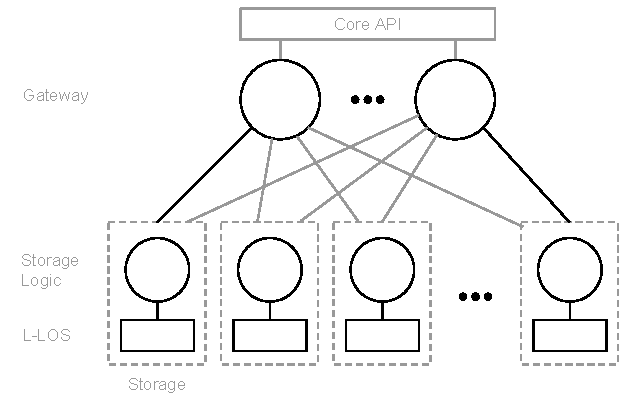
\includegraphics[scale=0.95]{pdf/sofa-llos-extension.pdf}
	\caption{L-LOS integration in \CodeName. \label{fig:sofa-llos-extension}}
\end{figure}

\section{Pipeline support}
A prioritized future implementation is to replace the Python Pyro4 communication library possible with one of the alternatives (Section \ref{sec:general}) that supports streaming to reduce the package latency, by implement the pipeline solution of the delegation framework (Section \ref{sec:delegation}) and the package distribution protocol in the append API call \ref{sec:api-append}.

\section{Parallel nodes} \label{sec:parallel}
As a consequence of the pipeline support and thereby the elimination of the existing communication library it is a demand and crucial for the future work to implement a proper protocol for handling multiple requests in parallel.

\section{Import/export extension}
Use \CodeName as a data transformation framework to unify data formats across multiple different input formats, by creating two new extensions for \CodeName at the same level as BDAE (Figure \ref{fig:bdae-extension}). The ambition is to create two generic self-awareness protocol-based data conversion frameworks where the end-users can specify input data\footnote{By url, path or other common formats.} and a result data format protocol such as HDF5 or NetCDF.

\begin{figure}
	\centering
	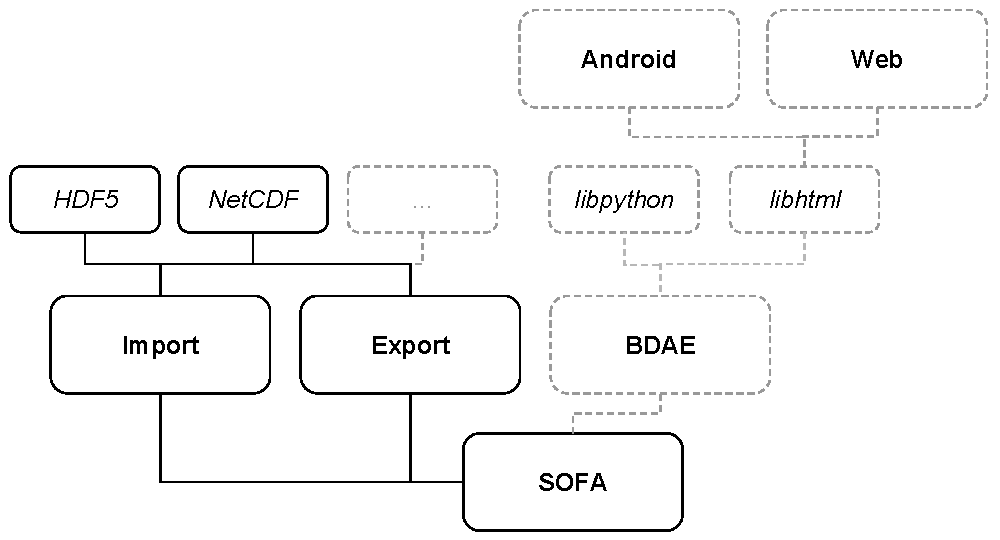
\includegraphics[scale=0.7]{pdf/bdae-extension.pdf}
	\caption{Import/export extension for \CodeName. \label{fig:bdae-extension}}
\end{figure}

\section{Security layer}
Implement an extended access protection layer opportunity at a dataset level by expanding the existing metadata structure with one of following two options:
\begin{enumerate}
	\item A public-key cryptography scheme such that it is only users with matching keys that have access to the data, such scheme is a way to identify trusted entities without involving password and used in protocols such as SSH.
	\item Maintaining a list of verified user identifiers and validate against it before any type operations involving the dataset.
\end{enumerate}

\section{Data encryption}
Implement an encryption/decryption layer which is optional to implement for the end-user and thus can be tailored specifically for individual dataset or applications. Such layer will facilitate options for storing and analyzing personally identifiable data out of the box in \CodeName. 
\newline

A straightforward solution extends the append flow (Figure \ref{fig:preprocess-nextentry}) such that each block is locally encrypted before distributed to the replicas. The decryption, on the other hand, has to be performed at a block level whenever an operation is executed.

\section{Enhanced benchmarks}
A final and evidently relevant task for the future is to implement an extended benchmark suite to compare \CodeName + BDAE against Hadoop and other big data analysis frameworks targeting the same audiences. The extensive comparison between the frameworks is only relevant whenever the rest of the optimizations and prioritized tasks described in this chapter has been applied.
